% A function f on [0,1] with the simple functions phi_1(f) and phi_3(f) below it (values cut into slices of height 2^-n). Generated by a short script.
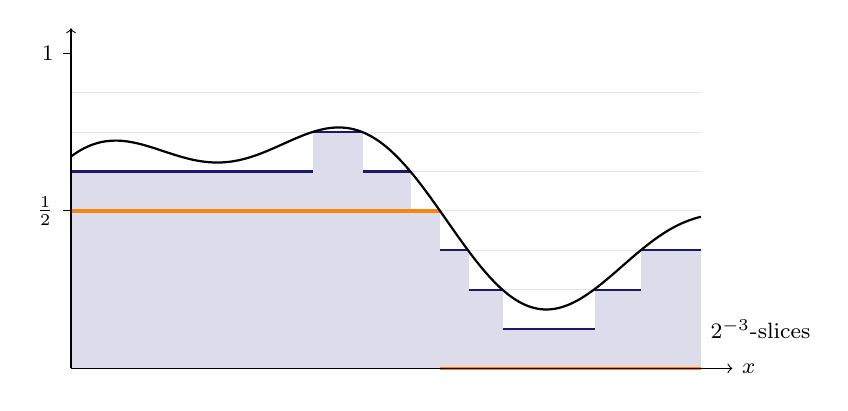
\begin{tikzpicture}[x=8.0cm,y=4.0cm]
\draw[black!10] (0,0.125)--(1,0.125);
\draw[black!10] (0,0.250)--(1,0.250);
\draw[black!10] (0,0.375)--(1,0.375);
\draw[black!10] (0,0.500)--(1,0.500);
\draw[black!10] (0,0.625)--(1,0.625);
\draw[black!10] (0,0.750)--(1,0.750);
\draw[black!10] (0,0.875)--(1,0.875);
\fill[MidnightBlue!15] (0.0000,0) rectangle (0.3837,0.6250);
\draw[MidnightBlue,thick] (0.0000,0.6250)--(0.3837,0.6250);
\fill[MidnightBlue!15] (0.3837,0) rectangle (0.4637,0.7500);
\draw[MidnightBlue,thick] (0.3837,0.7500)--(0.4637,0.7500);
\fill[MidnightBlue!15] (0.4637,0) rectangle (0.5400,0.6250);
\draw[MidnightBlue,thick] (0.4637,0.6250)--(0.5400,0.6250);
\fill[MidnightBlue!15] (0.5400,0) rectangle (0.5863,0.5000);
\draw[MidnightBlue,thick] (0.5400,0.5000)--(0.5863,0.5000);
\fill[MidnightBlue!15] (0.5863,0) rectangle (0.6312,0.3750);
\draw[MidnightBlue,thick] (0.5863,0.3750)--(0.6312,0.3750);
\fill[MidnightBlue!15] (0.6312,0) rectangle (0.6850,0.2500);
\draw[MidnightBlue,thick] (0.6312,0.2500)--(0.6850,0.2500);
\fill[MidnightBlue!15] (0.6850,0) rectangle (0.8313,0.1250);
\draw[MidnightBlue,thick] (0.6850,0.1250)--(0.8313,0.1250);
\fill[MidnightBlue!15] (0.8313,0) rectangle (0.9050,0.2500);
\draw[MidnightBlue,thick] (0.8313,0.2500)--(0.9050,0.2500);
\fill[MidnightBlue!15] (0.9050,0) rectangle (1.0000,0.3750);
\draw[MidnightBlue,thick] (0.9050,0.3750)--(1.0000,0.3750);
\draw[BurntOrange,very thick] (0.0000,0.5000)--(0.5863,0.5000);
\draw[BurntOrange,very thick] (0.5863,0.0000)--(1.0000,0.0000);
\draw[black,thick] plot coordinates {(0.0000,0.6727) (0.0050,0.6799) (0.0100,0.6865) (0.0150,0.6926) (0.0200,0.6980) (0.0250,0.7029) (0.0300,0.7073) (0.0350,0.7111) (0.0400,0.7143) (0.0450,0.7171) (0.0500,0.7193) (0.0550,0.7210) (0.0600,0.7222) (0.0650,0.7229) (0.0700,0.7232) (0.0750,0.7231) (0.0800,0.7225) (0.0850,0.7216) (0.0900,0.7203) (0.0950,0.7187) (0.1000,0.7168) (0.1050,0.7146) (0.1100,0.7122) (0.1150,0.7096) (0.1200,0.7067) (0.1250,0.7038) (0.1300,0.7006) (0.1350,0.6974) (0.1400,0.6942) (0.1450,0.6908) (0.1500,0.6875) (0.1550,0.6842) (0.1600,0.6810) (0.1650,0.6778) (0.1700,0.6747) (0.1750,0.6718) (0.1800,0.6690) (0.1850,0.6664) (0.1900,0.6639) (0.1950,0.6617) (0.2000,0.6597) (0.2050,0.6580) (0.2100,0.6566) (0.2150,0.6554) (0.2200,0.6545) (0.2250,0.6539) (0.2300,0.6536) (0.2350,0.6536) (0.2400,0.6540) (0.2450,0.6546) (0.2500,0.6556) (0.2550,0.6569) (0.2600,0.6585) (0.2650,0.6604) (0.2700,0.6626) (0.2750,0.6651) (0.2800,0.6678) (0.2850,0.6708) (0.2900,0.6741) (0.2950,0.6776) (0.3000,0.6813) (0.3050,0.6851) (0.3100,0.6892) (0.3150,0.6934) (0.3200,0.6977) (0.3250,0.7021) (0.3300,0.7065) (0.3350,0.7110) (0.3400,0.7155) (0.3450,0.7200) (0.3500,0.7244) (0.3550,0.7288) (0.3600,0.7330) (0.3650,0.7371) (0.3700,0.7411) (0.3750,0.7448) (0.3800,0.7483) (0.3850,0.7515) (0.3900,0.7545) (0.3950,0.7571) (0.4000,0.7594) (0.4050,0.7614) (0.4100,0.7629) (0.4150,0.7640) (0.4200,0.7647) (0.4250,0.7650) (0.4300,0.7647) (0.4350,0.7639) (0.4400,0.7627) (0.4450,0.7609) (0.4500,0.7585) (0.4550,0.7557) (0.4600,0.7522) (0.4650,0.7482) (0.4700,0.7436) (0.4750,0.7385) (0.4800,0.7327) (0.4850,0.7264) (0.4900,0.7196) (0.4950,0.7122) (0.5000,0.7042) (0.5050,0.6957) (0.5100,0.6866) (0.5150,0.6771) (0.5200,0.6670) (0.5250,0.6565) (0.5300,0.6455) (0.5350,0.6341) (0.5400,0.6223) (0.5450,0.6101) (0.5500,0.5975) (0.5550,0.5846) (0.5600,0.5715) (0.5650,0.5580) (0.5700,0.5444) (0.5750,0.5305) (0.5800,0.5165) (0.5850,0.5023) (0.5900,0.4881) (0.5950,0.4738) (0.6000,0.4595) (0.6050,0.4453) (0.6100,0.4310) (0.6150,0.4169) (0.6200,0.4030) (0.6250,0.3892) (0.6300,0.3756) (0.6350,0.3622) (0.6400,0.3492) (0.6450,0.3365) (0.6500,0.3241) (0.6550,0.3121) (0.6600,0.3005) (0.6650,0.2893) (0.6700,0.2786) (0.6750,0.2684) (0.6800,0.2588) (0.6850,0.2496) (0.6900,0.2411) (0.6950,0.2331) (0.7000,0.2257) (0.7050,0.2190) (0.7100,0.2128) (0.7150,0.2073) (0.7200,0.2025) (0.7250,0.1983) (0.7300,0.1948) (0.7350,0.1919) (0.7400,0.1897) (0.7450,0.1882) (0.7500,0.1872) (0.7550,0.1870) (0.7600,0.1874) (0.7650,0.1884) (0.7700,0.1900) (0.7750,0.1922) (0.7800,0.1950) (0.7850,0.1984) (0.7900,0.2022) (0.7950,0.2067) (0.8000,0.2116) (0.8050,0.2169) (0.8100,0.2227) (0.8150,0.2290) (0.8200,0.2356) (0.8250,0.2425) (0.8300,0.2498) (0.8350,0.2574) (0.8400,0.2652) (0.8450,0.2733) (0.8500,0.2815) (0.8550,0.2900) (0.8600,0.2985) (0.8650,0.3071) (0.8700,0.3159) (0.8750,0.3246) (0.8800,0.3333) (0.8850,0.3420) (0.8900,0.3507) (0.8950,0.3592) (0.9000,0.3677) (0.9050,0.3760) (0.9100,0.3841) (0.9150,0.3920) (0.9200,0.3997) (0.9250,0.4072) (0.9300,0.4144) (0.9350,0.4213) (0.9400,0.4279) (0.9450,0.4343) (0.9500,0.4403) (0.9550,0.4460) (0.9600,0.4513) (0.9650,0.4563) (0.9700,0.4609) (0.9750,0.4652) (0.9800,0.4691) (0.9850,0.4727) (0.9900,0.4759) (0.9950,0.4788) (1.0000,0.4813)};
\draw[->] (0,0)--(1.05,0) node[right,font=\footnotesize] {$x$};
\draw[->] (0,0)--(0,1.08);
\draw (0,0.5)--(-0.012,0.5) node[left,font=\footnotesize] {$\frac12$};
\draw (0,1)--(-0.012,1) node[left,font=\footnotesize] {$1$};
\node[right,font=\footnotesize] at (1.0,0.125) {$2^{-3}$-slices};
\end{tikzpicture}
